%
% File acl2015.tex
%
% Contact: car@ir.hit.edu.cn, gdzhou@suda.edu.cn
%%
%% Based on the style files for ACL-2014, which were, in turn,
%% Based on the style files for ACL-2013, which were, in turn,
%% Based on the style files for ACL-2012, which were, in turn,
%% based on the style files for ACL-2011, which were, in turn, 
%% based on the style files for ACL-2010, which were, in turn, 
%% based on the style files for ACL-IJCNLP-2009, which were, in turn,
%% based on the style files for EACL-2009 and IJCNLP-2008...

%% Based on the style files for EACL 2006 by 
%%e.agirre@ehu.es or Sergi.Balari@uab.es
%% and that of ACL 08 by Joakim Nivre and Noah Smith

\documentclass[11pt]{article}
\usepackage[labelfont=bf]{caption}
\usepackage{subcaption}
\usepackage{float}
\restylefloat{figure}
\usepackage{graphicx}
\usepackage{acl2015}
\usepackage{times}
\usepackage{url}
\usepackage{latexsym}
\usepackage{amsmath}
\usepackage{algorithmicx}
\usepackage{algpseudocode}
\usepackage{listings}
\usepackage[ruled]{algorithm}
\usepackage{multirow}
\usepackage{hyperref}
\hypersetup{
    colorlinks=true,
    linkcolor=black,
    filecolor=black,      
    urlcolor=blue,
}

%\setlength\titlebox{5cm}

% You can expand the titlebox if you need extra space
% to show all the authors. Please do not make the titlebox
% smaller than 5cm (the original size); we will check this
% in the camera-ready version and ask you to change it back.


\title{Prefix-Sum computation using OpenMP and MPI}

\author{Arun Krishnakumar Rajagopalan \\
  Texas A\&M University \\
  {\tt arunxls@gmail.com} \\}

\date{}

\begin{document}
\maketitle
\begin{abstract}
  Prefix sum calculation is among the most fundamental operations performed in parallel applications. In this paper, we look at two separate implementations of the Prefix sum algorithm and evaluate their performance against the most optimal sequential algorithm.
\end{abstract}

\section{Introduction}

Prefix sum is a useful primitive in several algorithms such as sorting, scheduling, graph algorithms etc. The prefix sum (also called a scan) of a sequence of numbers $x_{0}, x_{1}, x_{2},\ldots$ is defined as another sequence $y_{0}, y_{1}, y_{2},\ldots$ where

\begin{align*} 
y_{0} &= x_{0} \\ 
y_{1} &= x_{0} + x_{1} \\
y_{2} &= x_{0} + x_{1} + x_{2} \\
\ldots
\end{align*}

It is trivial to compute prefix sums in a sequential fashion. The rest of the paper discusses strategies to perform Prefix sums in parallel and report and analyze the results obtained. The paper continues as follows. Section 2 describes the theoretical analysis of the algorithms to compute prefix sums and their analysis. Section 3 describes the experimental setup. Section 4 contains evaluation of the parallel algorithm in comparison to its sequential counterpart. Section 5 contains concluding remarks and avenues for future improvement.

\section{Theoretical analysis}

In this paper, we discuss 3 separate implementations of Prefix sum - Sequential, OpenMP and MPI. 

\subsection{Sequential}

\renewcommand{\algorithmiccomment}[1]{// #1}
\begin{algorithm}
\caption{Sequential Prefix Sum}
\label{alg1}
\begin{algorithmic}[1]
  \State $X \leftarrow [x_{0}, x_{1}, \ldots, x_{n}]$
%   \Comment Input
  \State $Y \leftarrow \emptyset$
%   \Comment Output
  \State $Y[0] \leftarrow X[0]$
%   \Comment Initialize Y
  \For{i \textbf{from} 1 \textbf{to} N}
%   \Comment N is the size of X
    \State $Y[i] \leftarrow X[i] + Y[i-1]$
  \EndFor
  \State \Return Y
\end{algorithmic}
\end{algorithm}

The sequential algorithm is described by Algorithm \ref{alg1}. $X$ contains the array of input elements $[x_{0}, x_{1}, x_{2},\ldots, x_{N}]$. $Y$ stores the computes prefix sums. Line 3 initializes the first element of $Y$ to the first input element. Line 4 is the only loop in the algorithm. We iterate $N-1$ times, where $N$ refers to the size of the input array. At every loop iteration, we set $Y[i]$ to be the sum of the current input element and the previously computed sum $Y[i-1]$. Thus, at the end of each loop iteration, we end up with the correct prefix sum up to the iteration variable. 
\subsubsection{Complexity Analysis}

The loop at Line 4 determines the complexity of the algorithm since all other steps are constant $O(1)$ operations. The loop runs $N-1$ times and each operation inside the loop runs in $O(1)$ time. Thus, the total time complexity $T(n)$ is,

\[T(n) = O(n)\]


\subsection{MPI}
Message Passing Interface (MPI) is a language independent communications protocol used to program parallel computers in a distributed memory system. It supports both point-to-point and collective communication. 

\begin{algorithm}
\caption{MPI Prefix Sum}
\label{alg2}
\begin{algorithmic}[1]
  \State $X \leftarrow [x_{0}, x_{1}, \ldots, x_{n}]$
%   \Comment Input
  \For{N \textbf{in parallel}}
%   \Comment N is the size of X
      \State $id \leftarrow getId()$
    %   \Comment Get current process Id
      \For{h \textbf{from} 1 \textbf{to} $\log$ N}
        \If{$id > 2^{h-1}$}
            \State $x \leftarrow X[id - 2^{h-1}]$
            \State $y \leftarrow X[id]$
            \State $X[i] \leftarrow x + y$
        \Else
            \State \text{Exit}
        \EndIf
      \EndFor
    \EndFor
  \State \Return X
\end{algorithmic}
\end{algorithm}

The algorithm to compute prefix sums using MPI is described in Algorithm \ref{alg2}. Let X hold the input array. The algorithm computes the prefix sum in-place. N refers to the number of processing elements. For simplicity, let us assume that the total number of processing element equals the size of input. Section 2.4 will introduce a simple pre-processing and post-processing step that will help us lift this restriction. 

\begin{figure}[h!]
    \centering
        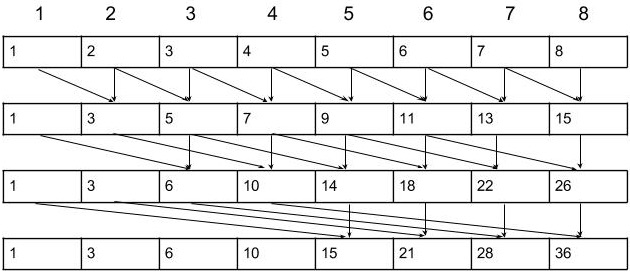
\includegraphics[scale=0.34]{MPI.jpg}
        \caption{An example of Algorithm \ref{alg2}}
        \label{fig1}
    \centering
\end{figure}

Line 2 runs the loop in parallel across N processing elements. Line 3 returns the processor ID, which runs from 1 to N. Each processor then executes the loop on Line 4 $\log N$ times. If the condition on Line 5 is not satisfied, that particular processor will exit early and stop any further computation. Lines 6-9 are where the main computation of prefix sums takes place.

Figure \ref{fig1} shows an application of this algorithm for an 8 element input size. The input elements run from 1 to 8. In each step of the algorithm, we notice that we have computed the prefix sums correctly up to $\log N$ elements.

This algorithm does not require that the number of processing nodes be a power of two. Thus, in cases where number of processors $\neq$ a power of two, we simply use the available processors and bound check appropriately so that we don't access an illegal memory location.

\subsubsection{Complexity Analysis}
The running time of the algorithm is governed by the loop on Line 4. Each operation inside the loop takes constant time, hence the total running time is \(T(n) = O(\log n)\).

\noindent The total work done can be calculated as (total number of active processors at each iteration) $\times$ (work done per processor at each iteration). However, the work done at each iteration is O(1). Thus, 
\begin{align*} 
W(n) &= \sum\limits_{i=1}^{\log n} n + 1 - 2^{i - 1}  \\ 
&= n{\log n} - \sum\limits_{i=1}^{\log n} 2^{i - 1}  \\
&= n{\log n} - n  \\
&= O(n\log n)  \\
\end{align*}

\subsection{OpenMP}
OpenMP is a framework to program parallel applications in a shared memory model. The program starts off with a master thread which then forks off slave threads who each divide the work among themselves. The threads then run concurrently on different processors allocated by the runtime environment.

\begin{algorithm}
\caption{OpenMP Prefix Sum}
\label{alg3}
\begin{algorithmic}[1]
  \State $X \leftarrow [x_{0}, x_{1}, \ldots, x_{n}]$
%   \Comment Input
  \State \Comment SweepUp
  \For{h \textbf{from} 0 \textbf{to} $\log$ N - 1}
%   \Comment N is the size of X
    %   \Comment Get current process Id
      \For{i \textbf{from} 0 \textbf{to} $N/2^{h+1}$ \textbf{in parallel}}
        \State $a \leftarrow 2^{h+1} \times (i+1) - 1$
        \State $b \leftarrow a - 2^{h}$
        \State $X[a] \leftarrow X[a] + X[b]$
      \EndFor
    \EndFor
    \State
    \State \Comment SweepDown
    \State $X[N-1] \leftarrow 0$
    % \Comment Set the last element to 0
    \For{h \textbf{from} $\log$ N - 1 \textbf{to} 0}
      \For{i \textbf{from} 0 \textbf{to} $N/2^{h+1}$ \textbf{in parallel}}
        \State $a \leftarrow 2^{h+1} \times (i+1) - 1$
        \State $b \leftarrow a - 2^{h}$
        \State $temp \leftarrow X[a]$
        \State $X[a] \leftarrow X[a] + X[b]$
        \State $X[b] \leftarrow temp$
      \EndFor
    \EndFor

\end{algorithmic}
\end{algorithm}

\begin{figure*}[t]
    \centering
    \begin{subfigure}[h!]{0.49\textwidth}
        \centering
        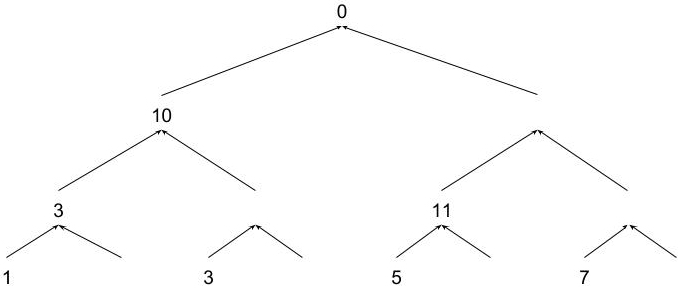
\includegraphics[width=\textwidth]{sweepDown2}
        \caption{After inserting 0}
        \label{fig:TA}
    \end{subfigure}
    \hfill
    \begin{subfigure}[h!]{0.49\textwidth}
        \centering
        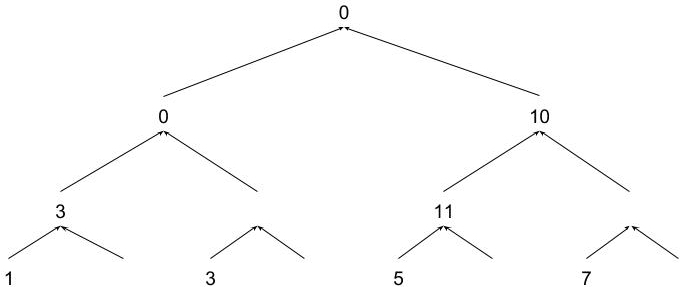
\includegraphics[width=\textwidth]{sweepDown3}
        \caption{After Iteration 1}
        \label{fig:TB}
    \end{subfigure}
    \hfill
    \begin{subfigure}[h!]{0.49\textwidth}
        \centering
        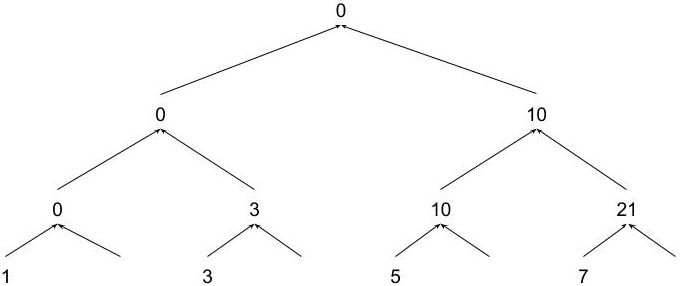
\includegraphics[width=\textwidth]{sweepDown4}
        \caption{After Iteration 2}
        \label{fig:TC}
    \end{subfigure}
    \hfill
    \begin{subfigure}[h!]{0.49\textwidth}
        \centering
        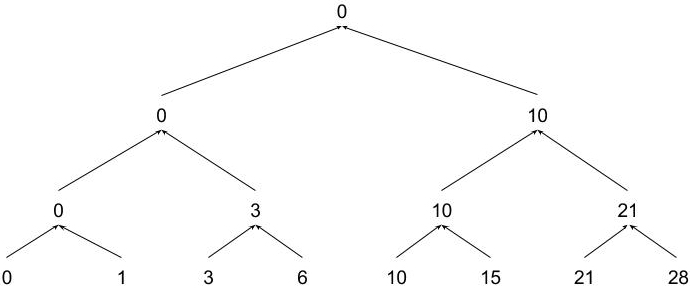
\includegraphics[width=\textwidth]{sweepDown5}
        \caption{After Iteration 3}
        \label{fig:TD}
    \end{subfigure}
    \caption{These 4 figures represent how the tree would look at the end of each iteration}
    \label{fig: Diff_traces}
\end{figure*}

The algorithm to compute Prefix Sums using OpenMP is described in Algorithm \ref{alg3}. The main idea of this algorithm is to visualize the input array as a balanced binary tree and work on it two phases - a `sweepUp' where we go from the bottom leaves to the root and a `sweepDown', where we do the reverse.

The sweepUp phase is similar to parallel sum algorithm. At the end of this phase, the last element hold the overall sum of the input sequence. 

\begin{figure}[h!]
    \centering
        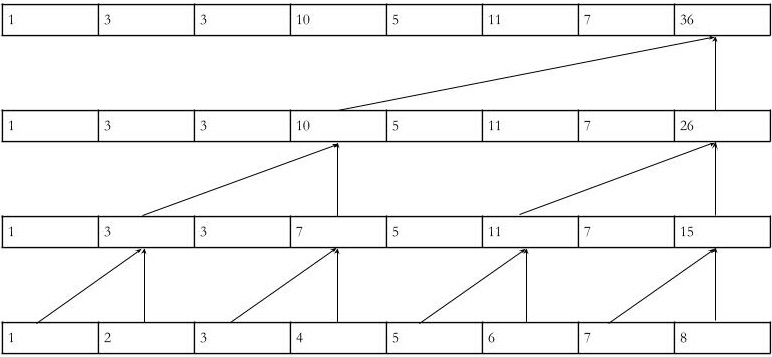
\includegraphics[scale=0.28]{sweepUp.jpg}
        \caption{An example after the sweepUp Phase}
        \label{fig2}
    \centering
\end{figure}

After completion of the sweepUp phase, we start the sweepDown phase. We treat the array as a balanced binary tree. The tree is constructed in such a way that the left children are all filled with values and the right children are empty. They will be filled with values as the algorithm proceeds. We start with the root and work our way down to the leaves. The root element is given the value 0 to begin with. At this stage, the tree would look like Figure \ref{fig:TA}. Subsequent stages of the algorithm are shown in Figure \ref{fig:TB}, \ref{fig:TC}, \ref{fig:TD}. At the end of this phase, we have the correct prefix sums calculated for each element.

In case the number of processors is not a multiple of two, we perform a clever manipulation taking advantage of shared memory. First, pad the input array with the enough zeros to get it to the next power of two. Then, we perform prefix sum as we would normally, but this time only using $p$ processors. Since the extra elements were initialized to 0, the correct value of prefix sum is calculated at the end.

\subsubsection{Complexity Analysis}
The running time of the algorithm is bounded by the running time of the sweepUp phase + the running time of the sweepDown phase. From Algorithm \ref{alg3}, we can see that both the phases run $\log n$ number of times, and each iteration takes constant time. Thus, the total running time is
\begin{align*} 
T(n) &= O(\log n) + O(\log n)  \\ 
&= O(\log n)  \\
\end{align*}

\noindent The total work done can be calculated as the sum of the work done by the sweepUp phase and the work done by the sweepDown phase. The work done by the sweepUp phase can be calculated as (total number of active processors at each iteration) $\times$ (work done per processor at each iteration). However, the work done at each iteration is O(1). Thus,
\begin{align*} 
W(n) &= \sum\limits_{k=1}^{\log n} \frac{n}{2^{k}}  \\ 
&= n\times\bigg(\frac{1}{2^{1}} + \frac{1}{2^{2}} + \ldots + \frac{1}{2^{\log n}}\bigg)  \\
&= O(\log n)  \\
\end{align*}

The work complexity for the sweepDown phase is identical to the sweepUp phase. Thus, the total work is \(W(n) = O(n)\). This is equal to the complexity of the sequential algorithm, making the algorithm work-optimal.

\subsection{Local Prefix Sum}

Algorithms \ref{alg2} and Algorithm \ref{alg3} work well for when the number of input elements equals the number of processing cores available. However, unless the input is trivial, the number of input elements (n) $\gg$ number of processing elements (p). In such cases, the input is divided up into chunks of $\frac{n}{p}$ size. Each processing element is assignment one of these chunks. The modified algorithm now computes the `local Prefix Sum' of each of these chunks. Once computed, the last prefix sum calculated within each chunk is then sent to be processed according to either Algorithm \ref{alg2} or Algorithm \ref{alg3}. Once we return from the parallel prefix-sum call, we then need to apply the appropriate offsets to each of the $\frac{n}{p}$ sections. The final result would be the correct computation of prefix sum for $n$ input elements and $p$ processing nodes. 

\begin{algorithm}
\caption{Local Prefix Sum}
\label{alg4}
\begin{algorithmic}[1]
  \State $X \leftarrow [x_{0}, x_{1}, \ldots, x_{n}]$
  \State $P \leftarrow [p_{0}, p_{1}, \ldots, p_{n}]$
  \State
  \For{N \textbf{in parallel}}
%   \Comment N is the size of X
      \State $id \leftarrow getId()$
    %   \Comment Get current process Id
      \For{i \textbf{from} $(id\times\frac{n}{p}) + 1$ \textbf{to} $(id + 1)\times\frac{n}{p}$}
        \State $X[i] \leftarrow X[i] + X[i - 1]$
      \EndFor
      \State $Y[i] \leftarrow X[(id + 1)\times\frac{n}{p}]$
    \EndFor
    \State
    \State $ParallelPrefixSum(Y[])$
    \State
    \For{N \textbf{in parallel}}
%   \Comment N is the size of X
      \State $id \leftarrow getId()$
    %   \Comment Get current process Id
      \For{i \textbf{from} $(id\times\frac{n}{p}) + 1$ \textbf{to} $(id + 1)\times\frac{n}{p}$}
        \State $X[i] \leftarrow X[i] + Y[id]$
      \EndFor
    \EndFor
\end{algorithmic}
\end{algorithm}

\subsubsection{Complexity}

\begin{table*}
\setlength{\tabcolsep}{15pt}
    \begin{center}
    \begin{tabular}{|c|c|c|c|c|c|}
    \hline
    \multirow{2}{*}{\textbf{Number of Processors}} & \multicolumn{5}{c|}{\textbf{Input Size} \emph{($\times10^{9}$)}} \\ \cline{2-6}
                         & \textbf{1} & \textbf{2} & \textbf{4} & \textbf{8} & \textbf{16} \\ \hline
    1                    & 0.297    & 0.595    & 1.193    & 2.407    & 4.907 \\ \hline
    2                    & 0.281	   & 0.567    & 1.132    & 2.262    & 4.514 \\ \hline
    4                    & 0.164    & 0.331    & 0.665    & 1.337    & 2.732 \\ \hline
    8                    & 0.119    & 0.238    & 0.511    & 1.072    & 2.212 \\ \hline
    12                   & 0.130   & 0.256    & 0.502    & 1.026    & 2.087 \\ \hline
    \end{tabular}
    \end{center}
    \caption{OpenMP implementation of Prefix Sum. All values of time are in seconds.}
    
    \begin{center}
    \begin{tabular}{|c|c|c|c|c|c|}
    \hline
    \multirow{2}{*}{\textbf{Number of Processors}} & \multicolumn{5}{c|}{\textbf{Input Size} \emph{($\times10^{9}$)}} \\ \cline{2-6}
                         & \textbf{1} & \textbf{2} & \textbf{4} & \textbf{8} & \textbf{16} \\ \hline
    1                    & 0.298    & 0.549    & 1.096    & 1.329    & 3.001 \\ \hline
    2                    & 0.140	& 0.280    & 0.560    & 1.115    & 2.221 \\ \hline
    4                    & 0.106    & 0.209    & 0.426    & 0.852    & 1.702 \\ \hline
    8                    & 0.098    & 0.198    & 0.397    & 0.796    & 1.601 \\ \hline
    16                   & 0.048    & 0.097    & 0.211    & 0.424    & 0.793 \\ \hline
    32                   & 0.024    & 0.048    & 0.096    & 0.198    & 0.390 \\ \hline
    64                   & 0.012    & 0.025    & 0.050    & 0.099    & 0.226 \\ \hline
    128                  & 0.006    & 0.013    & 0.026    & 0.052    & 0.100 \\ \hline
    \end{tabular}
    \end{center}
    \caption{MPI implementation of Prefix Sum. All values of time are in seconds.}
    
\end{table*}


\begin{figure*}[t]
    \centering
    \begin{subfigure}[h!]{0.3\textwidth}
        \centering
        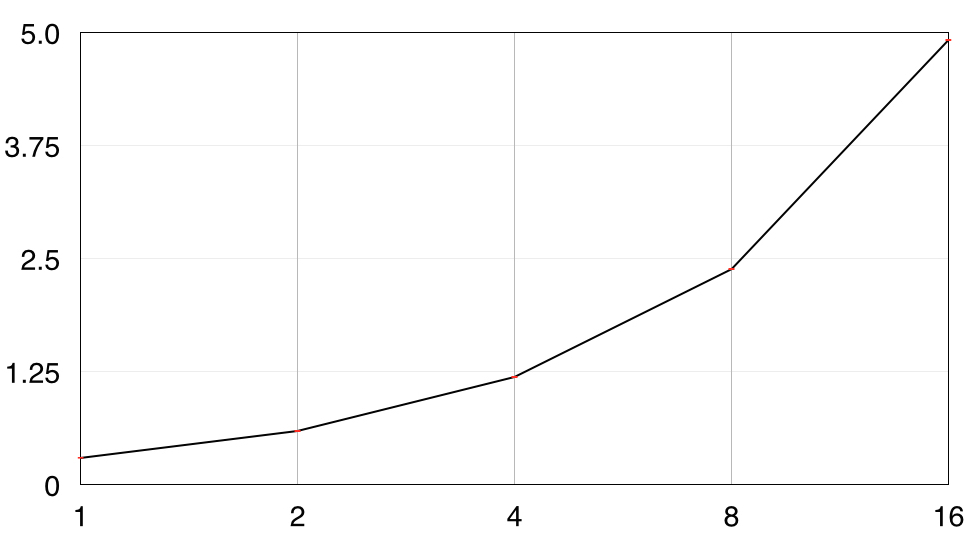
\includegraphics[width=4.5cm,height=5cm,keepaspectratio]{o1}
        \caption{OpenMP 1-thread}
        % \label{fig:TA}
    \end{subfigure}
    \hfill
    \begin{subfigure}[h!]{0.3\textwidth}
        \centering
        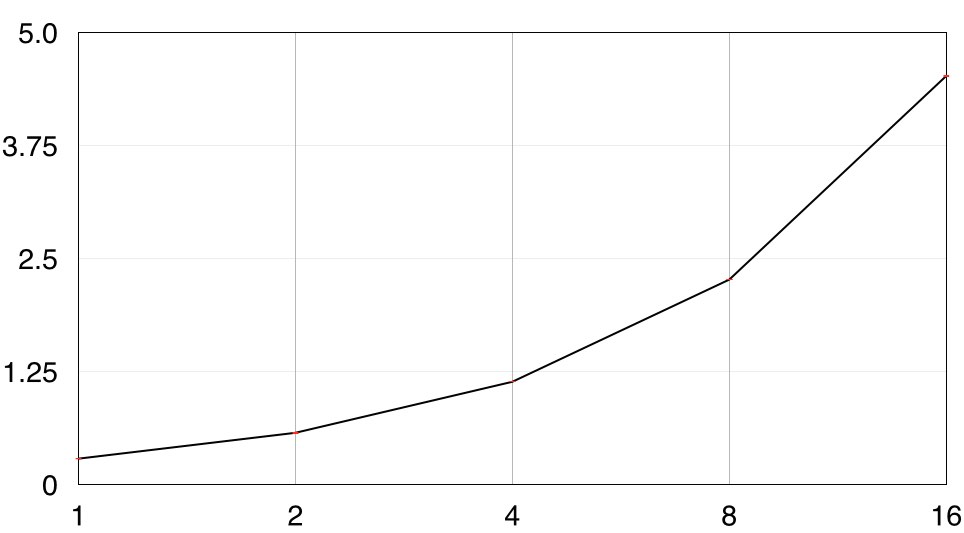
\includegraphics[width=4.5cm,height=5cm,keepaspectratio]{o2}
        \caption{OpenMP 2-thread}
        % \label{fig:TA}
    \end{subfigure}
    \hfill
    \begin{subfigure}[h!]{0.3\textwidth}
        \centering
        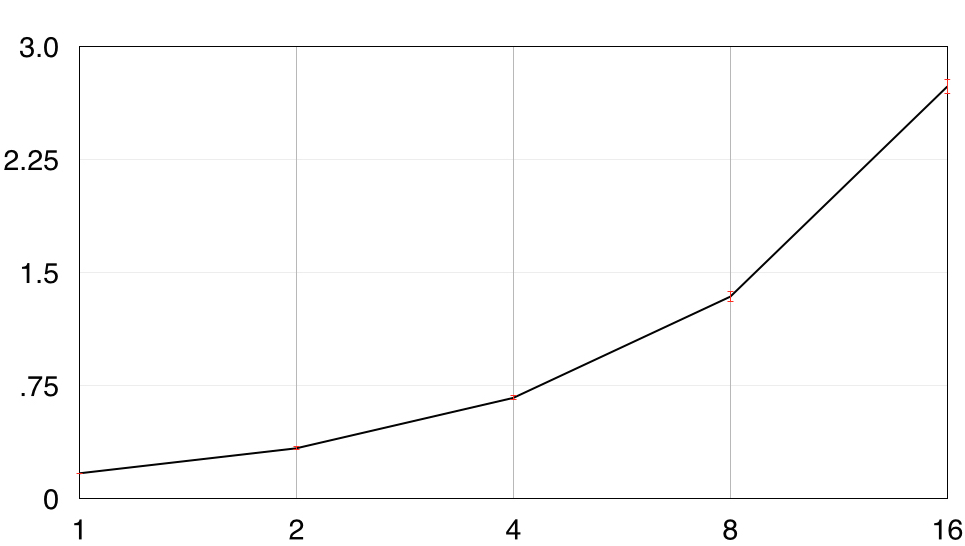
\includegraphics[width=4.5cm,height=5cm,keepaspectratio]{o4}
        \caption{OpenMP 4-thread}
        % \label{fig:TA}
    \end{subfigure}
    \hfill
    \begin{subfigure}[h!]{0.3\textwidth}
        \centering
        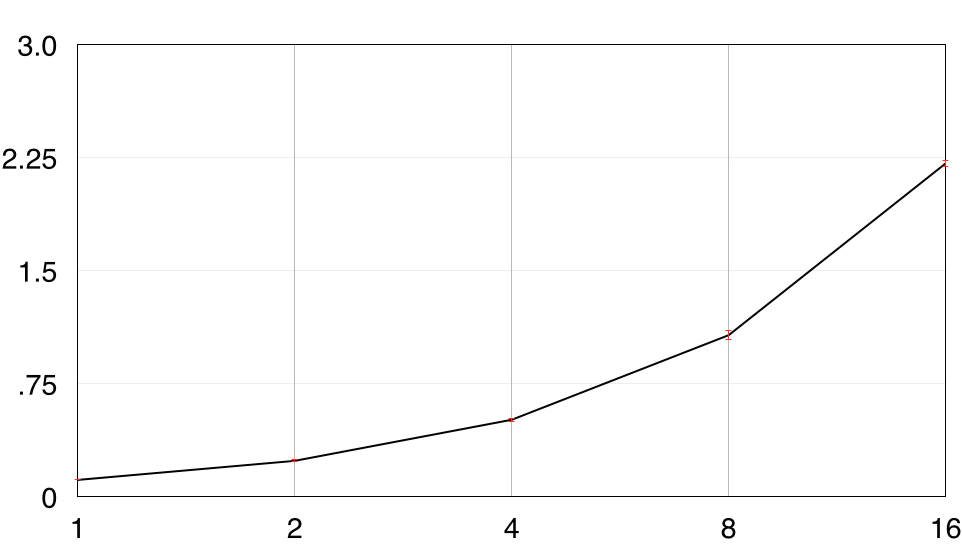
\includegraphics[width=4.5cm,height=5cm,keepaspectratio]{o8}
        \caption{OpenMP 8-thread}
        % \label{fig:TA}
    \end{subfigure}
    \hfill
    \begin{subfigure}[h!]{0.3\textwidth}
        \centering
        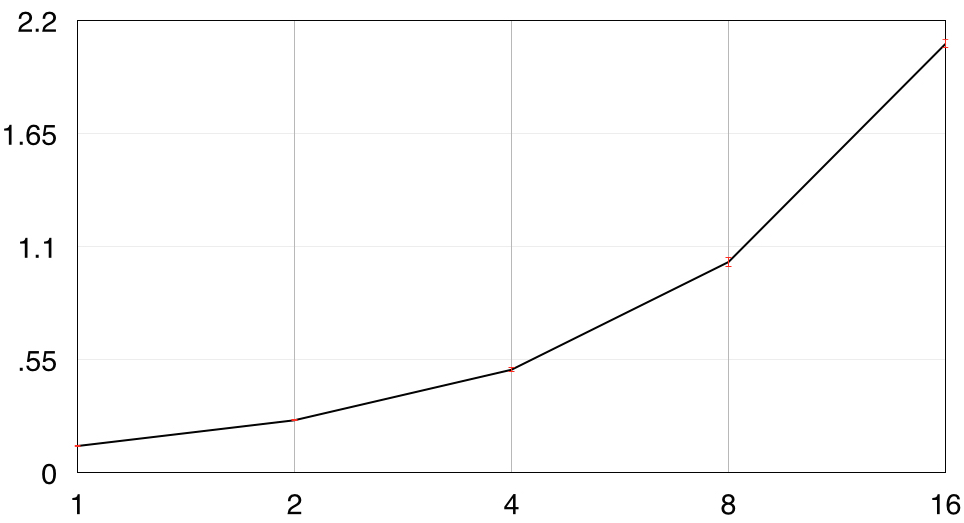
\includegraphics[width=4.5cm,height=5cm,keepaspectratio]{o12}
        \caption{OpenMP 12-thread}
        % \label{fig:TA}
    \end{subfigure}
    \hfill
    \begin{subfigure}[h!]{0.3\textwidth}
        \centering
        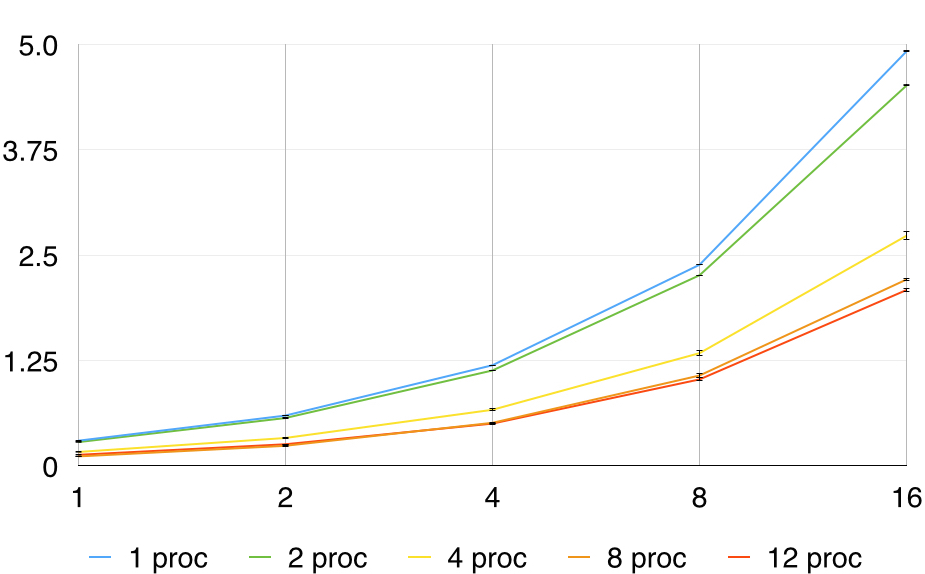
\includegraphics[width=4.5cm,height=5cm,keepaspectratio]{OpenMP_Comp}
        \caption{OpenMP Thread Comparison}
        % \label{fig:TA}
    \end{subfigure}
    \hfill
    \caption{Performance of OpenMP Prefix Sum. The X axis for all figures represents $10^{9}$ integers and the Y axis represents seconds.}
\end{figure*}

\begin{figure*}[ht]
    \centering
        \begin{subfigure}[h!]{0.3\textwidth}
        \centering
        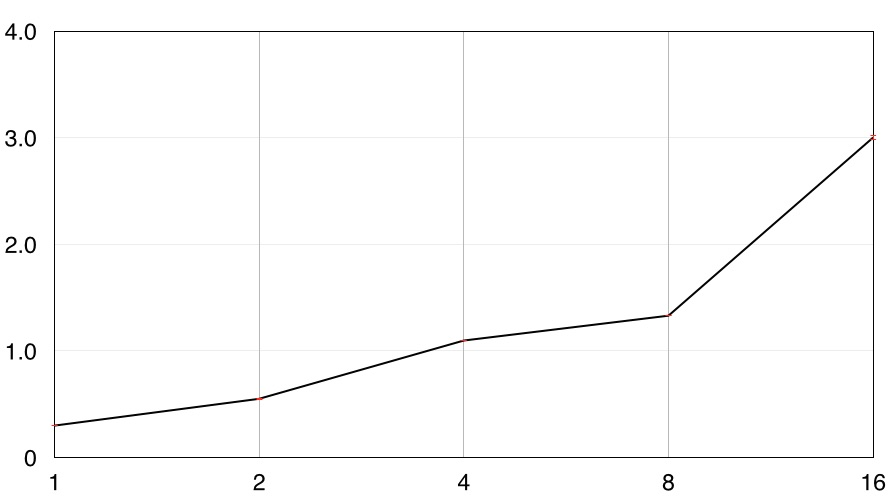
\includegraphics[width=4.5cm,height=5cm,keepaspectratio]{m1}
        \caption{MPI 1-node}
        % \label{fig:TA}
    \end{subfigure}
    \hfill
    \begin{subfigure}[h!]{0.3\textwidth}
        \centering
        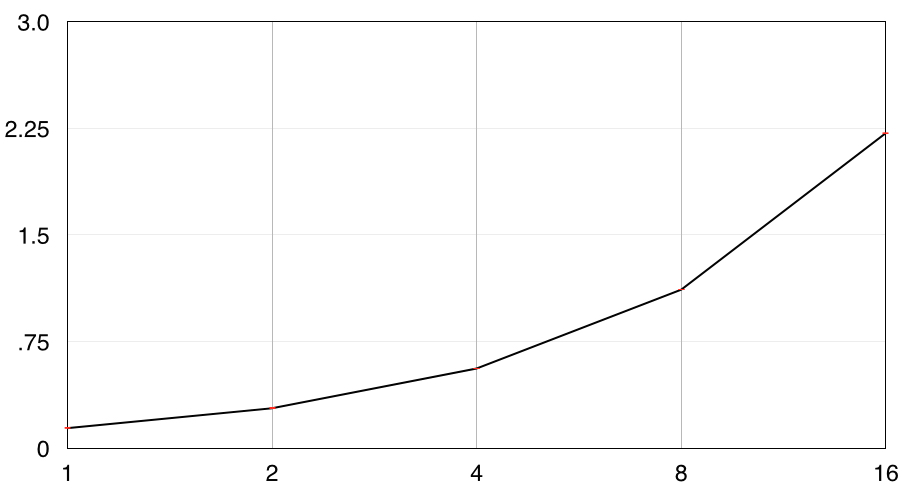
\includegraphics[width=4.5cm,height=5cm,keepaspectratio]{m2}
        \caption{MPI 2-node}
        % \label{fig:TA}
    \end{subfigure}
    \hfill
    \begin{subfigure}[h!]{0.3\textwidth}
        \centering
        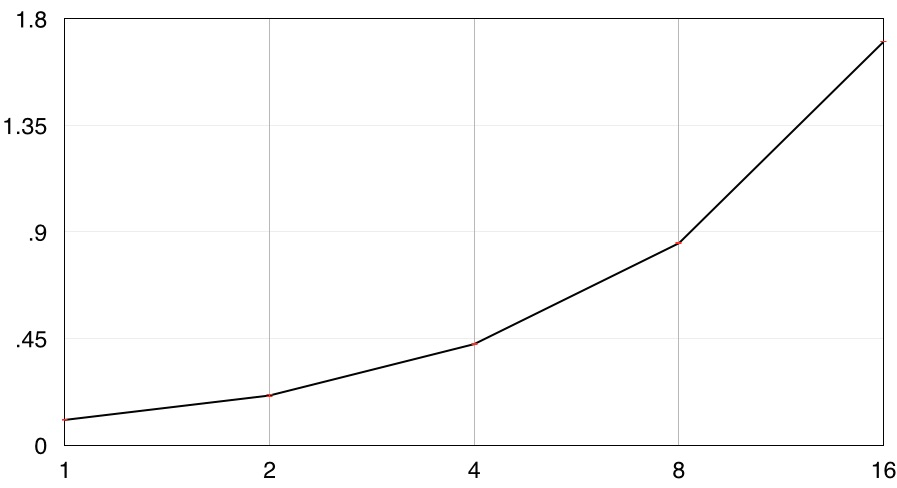
\includegraphics[width=4.5cm,height=5cm,keepaspectratio]{m4}
        \caption{MPI 4-node}
        % \label{fig:TA}
    \end{subfigure}
    \hfill
    \begin{subfigure}[h!]{0.3\textwidth}
        \centering
        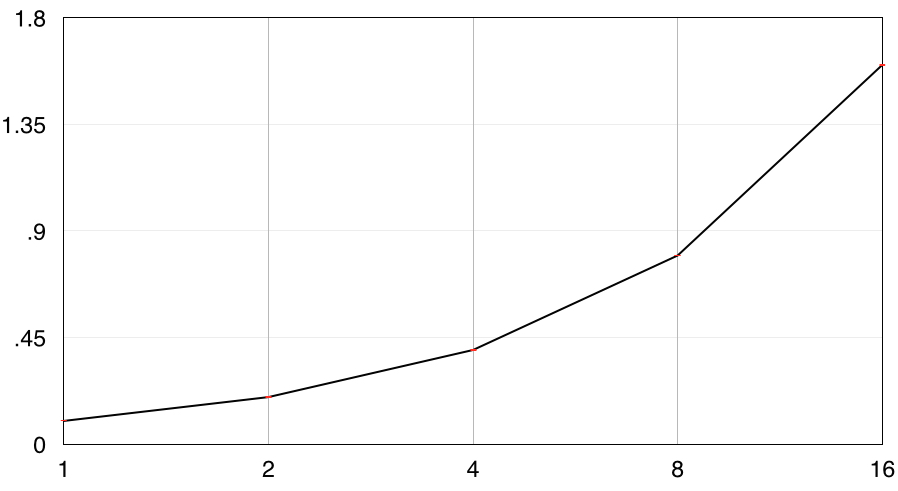
\includegraphics[width=4.5cm,height=5cm,keepaspectratio]{m8}
        \caption{MPI 8-node}
        % \label{fig:TA}
    \end{subfigure}
    \hfill
    \begin{subfigure}[h!]{0.3\textwidth}
        \centering
        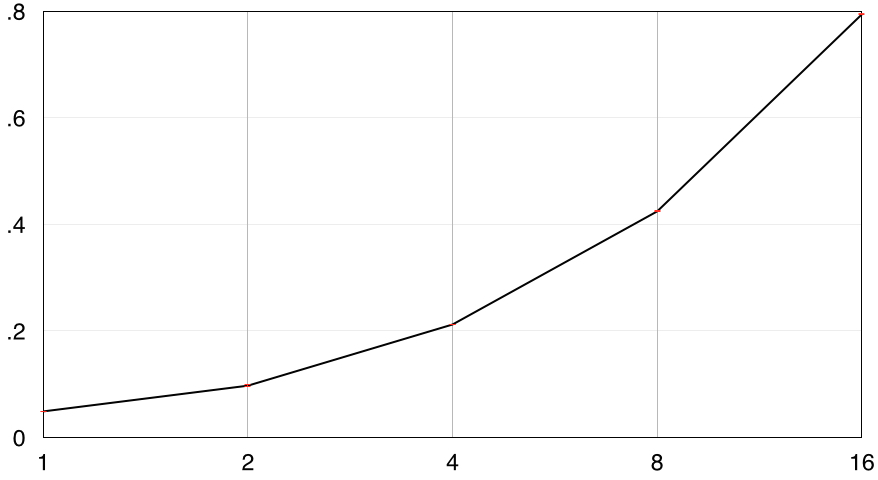
\includegraphics[width=4.5cm,height=5cm,keepaspectratio]{m16}
        \caption{MPI 16-node}
        % \label{fig:TA}
    \end{subfigure}
    \hfill
    \begin{subfigure}[h!]{0.3\textwidth}
        \centering
        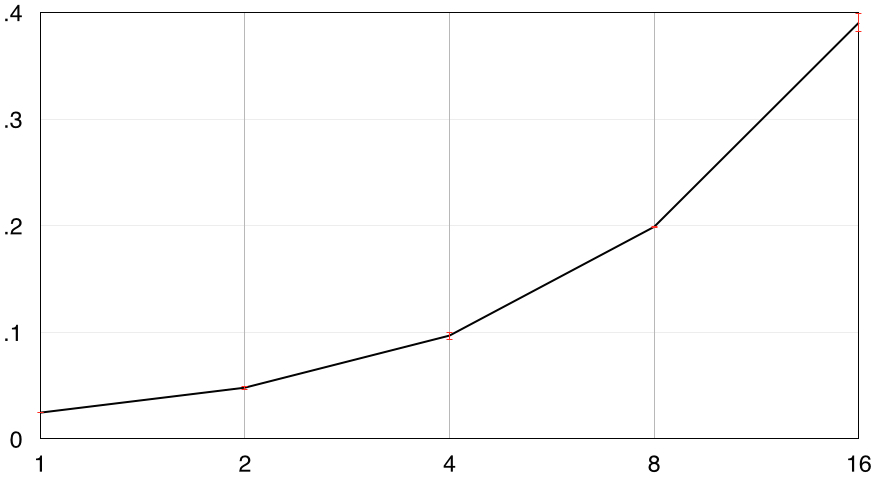
\includegraphics[width=4.5cm,height=5cm,keepaspectratio]{m32}
        \caption{MPI 32-node}
        % \label{fig:TA}
    \end{subfigure}
    \hfill
    \begin{subfigure}[h!]{0.3\textwidth}
        \centering
        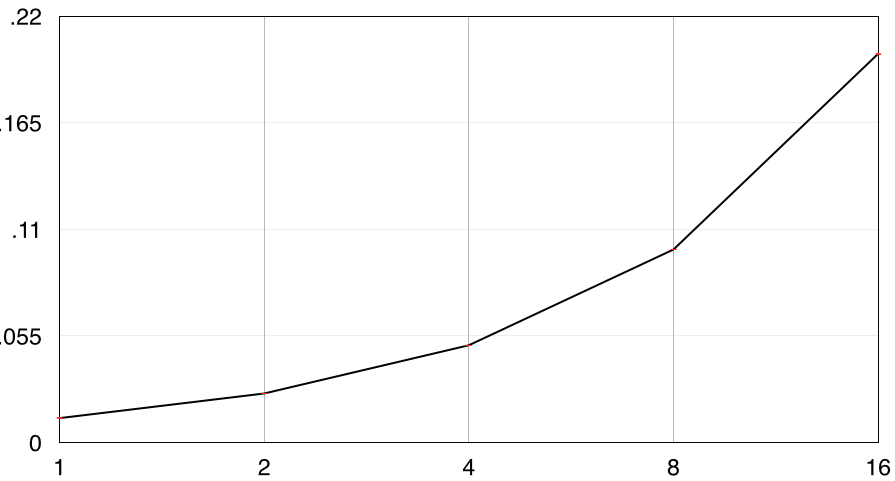
\includegraphics[width=4.5cm,height=5cm,keepaspectratio]{m64}
        \caption{MPI 64-node}
        % \label{fig:TA}
    \end{subfigure}
    \hfill
    \begin{subfigure}[h!]{0.3\textwidth}
        \centering
        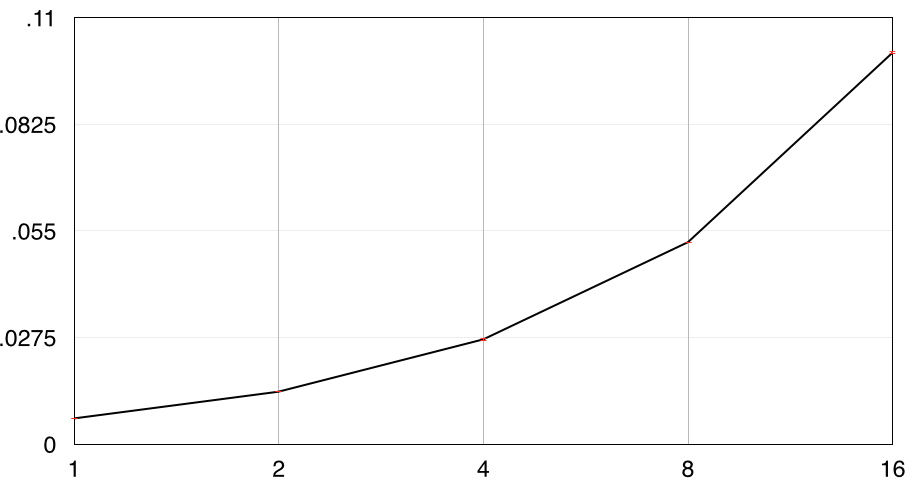
\includegraphics[width=4.5cm,height=5cm,keepaspectratio]{m128}
        \caption{MPI 128-node}
        % \label{fig:TA}
    \end{subfigure}
    \hfill
    \begin{subfigure}[h!]{0.3\textwidth}
        \centering
        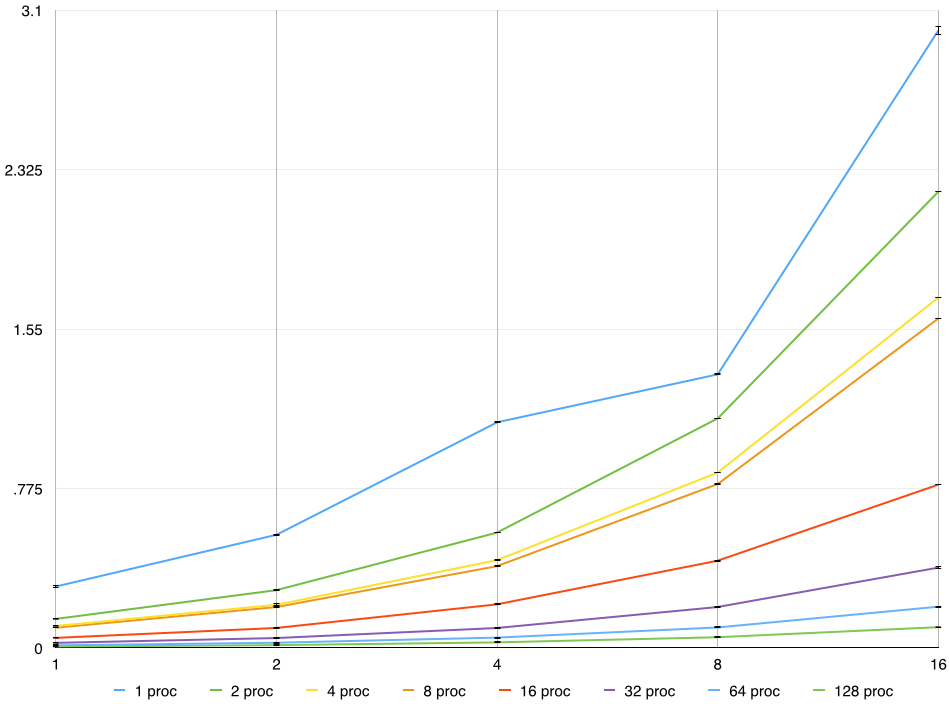
\includegraphics[width=4.5cm,height=5cm,keepaspectratio]{MPI_Comp}
        \caption{MPI Node Comparison}
        % \label{fig:TA}
    \end{subfigure}
    \hfill
    \caption{Performance of MPI Prefix Sum. The X axis for all figures represents $10^{9}$ integers and the Y axis represents seconds.}
\end{figure*}

\begin{figure*}[ht]
    \centering
    \begin{subfigure}[h!]{0.3\textwidth}
        \centering
        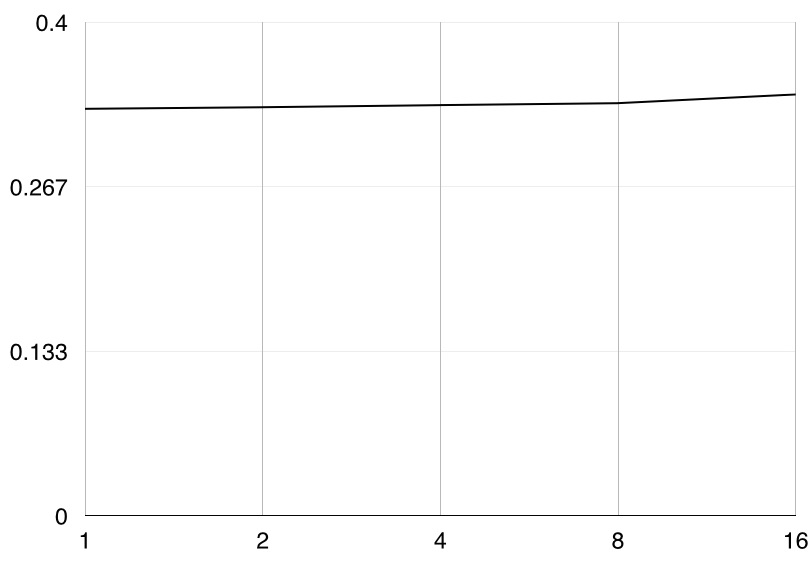
\includegraphics[width=4.5cm,height=5cm,keepaspectratio]{o_c4}
        \caption{OpenMP 4-threads}
        \label{fig:C4}
    \end{subfigure}
    \hfill
    \begin{subfigure}[h!]{0.3\textwidth}
        \centering
        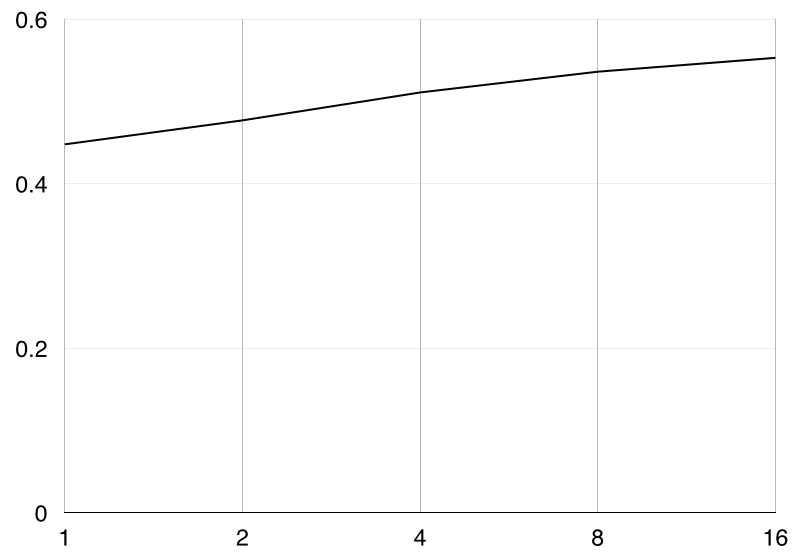
\includegraphics[width=4.5cm,height=5cm,keepaspectratio]{o_c8}
        \caption{OpenMP 8-threads}
        \label{fig:C8}
    \end{subfigure}
    \hfill
    \begin{subfigure}[h!]{0.3\textwidth}
        \centering
        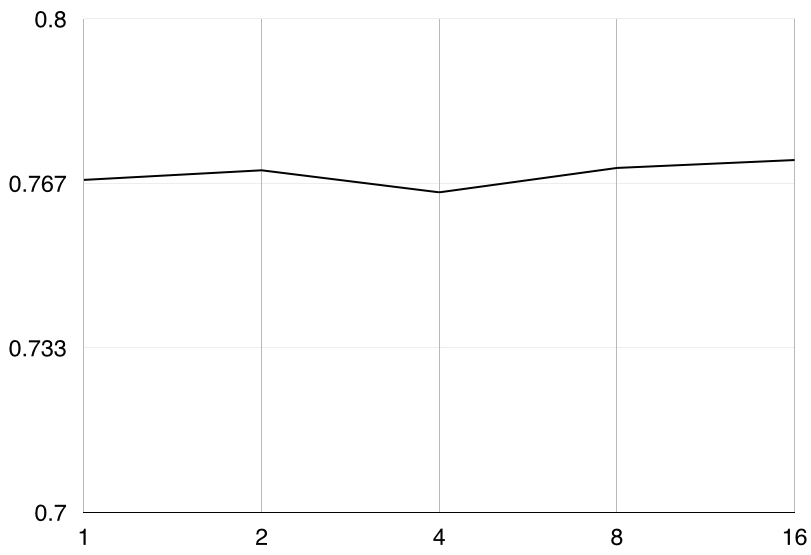
\includegraphics[width=4.5cm,height=5cm,keepaspectratio]{o_c12}
        \caption{OpenMP 12-threads}
        \label{fig:C12}
    \end{subfigure}
    \hfill
    \begin{subfigure}[h!]{0.3\textwidth}
        \centering
        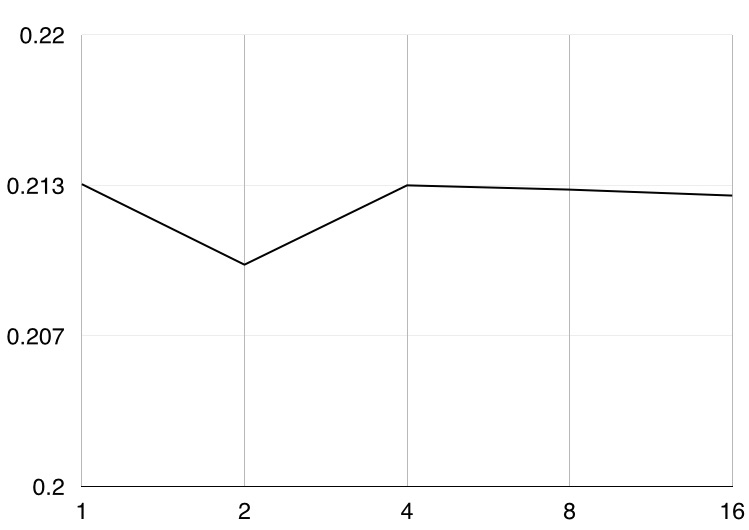
\includegraphics[width=4.5cm,height=5cm,keepaspectratio]{m_4}
        \caption{MPI 4-nodes}
        \label{fig:M4}
    \end{subfigure}
    \hfill
    \begin{subfigure}[h!]{0.3\textwidth}
        \centering
        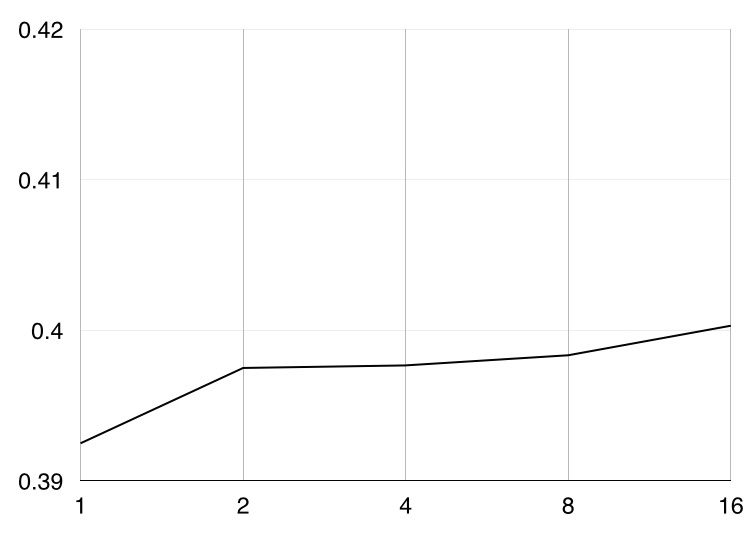
\includegraphics[width=4.5cm,height=5cm,keepaspectratio]{m_8}
        \caption{MPI 8-nodes}
        \label{fig:M8}
    \end{subfigure}
    \hfill
    \begin{subfigure}[h!]{0.3\textwidth}
        \centering
        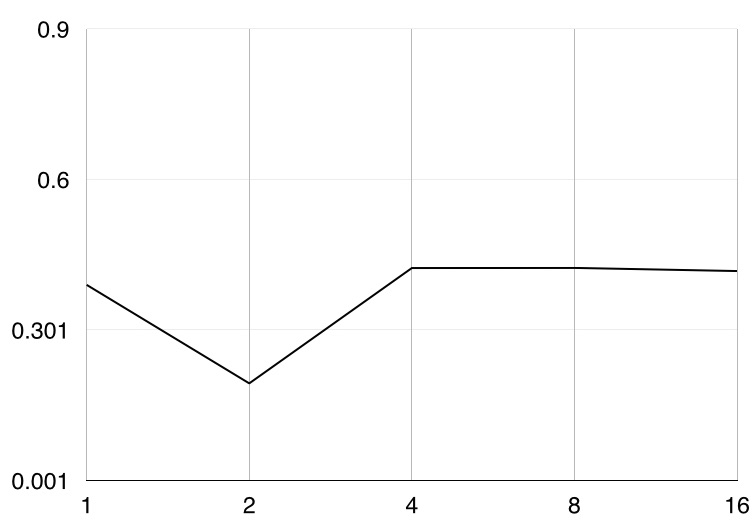
\includegraphics[width=4.5cm,height=5cm,keepaspectratio]{m_16}
        \caption{MPI 16-nodes}
        \label{fig:M16}
    \end{subfigure}
    \hfill
    \label{Constants}
    \caption{Algorithm constant determination. The X axis for all figures represents $10^{9}$ integers and the Y axis represents seconds.}
\end{figure*}

The algorithm consists of three phases - the first phase where were compute the local prefix sum, the second phase where we calculate the parallel prefix sums across processors and the last step where wer calculate the actual prefix sum from the offsets of the previous step. Thus, the overall time complexity $T(n)$ is,

\[T(n) = T_{1}(n) + T_{2}(n) + T_{3}(n)\]

Both $T_{1}(n)$ and $T_{3}(n)$ are similar to the sequential prefix sum (Algorithm \ref{alg1}) and share the same time complexity $O(N)$. In this case, $N = \frac{n}{p}$. $T_{2}(n)$ represents the time complexity of the parallel prefix sum step, which as we have seen in Algorithm \ref{alg2} and Algorithm \ref{alg3} is $O(\log N)$. In this case, $N = p$. The overall complexity is

\begin{align*} 
T(n) &= O\bigg(\frac{n}{p}\bigg) + O(\log p) + O\bigg(\frac{n}{p}\bigg) \\ 
&= O\bigg(\frac{n}{p}\bigg) + O(\log p) \\
\end{align*}

For very large inputs, $O(\frac{n}{p}) \gg O(\log p)$.

\section{Experimental Setup}

This section contains various details regarding the experimental setup and the test environment.

\subsection{Machine specification}

All experiments were run on the \textbf{EOS} super-computer, located at Texas A\&M. EOS is an IBM iDataPlex commodity cluster with nodes based on Intel's 64-bit Nehalem and Westmere processor. The cluster is composed of 372 compute nodes (324 8-way Nehalem- and 48 12-way Westmere-based). The compute nodes each have 24 GB of DDR3 1333 MHz memory.

\subsection{Test cases}

Various experiments were run against the three algorithms explained in Section 2. For each experimental run, the input size, run time and number of processors (where applicable) were noted.

\subsubsection{Input Data}

The input data is generated by a call to $rand()$ after seeding it with the current processor's ID and current time-stamp. This ensures we get a random data set for each run. Each program was run on input sizes of 1, 2, 4, 8 and 16 billion integers.

\subsubsection{Run time}

The execution time for each run is measured using $gettimeofday()$ method. The overhead of using this function is in the order of $10-100 ns$. Since the granularity of data needed is orders of magnitude larger, this function works well for these experiments. To get a higher expected confidence in the measured data, each experiment was run 32 times and the average runtime was taken.

\subsubsection{MPI}

All the MPI experiments were run on 1, 2, 4, 8, 12, 32 and 64 nodes. 

\subsubsection{OpenMP}

All the OpenMP experiments were run on 1, 2, 4, 8 and 12 core machines. The experiments were run such that there was 1 thread per core.

\section{Evaluation}

Various analysis on the observed data were carried out. In general, it was observed that the execution time for a given model reduced as we increased the number of processors in both models.

\subsection{Speed Up}

In this analysis, we measure the speedup achieved by the algorithm with respect to the sequential program, given by $\frac{T_{s}}{T_{p}}$, where $T_{s}$ represents the time of sequential program and $T_{p}$ represents the parallel implementation.Figure \ref{SpeedUp_MPI} and Figure \ref{SpeedUp_OpenMP} graph the speedup characteristics of both versions of prefix sum algorithm against 16 billions integers.

\begin{figure}[h!]
    \centering
        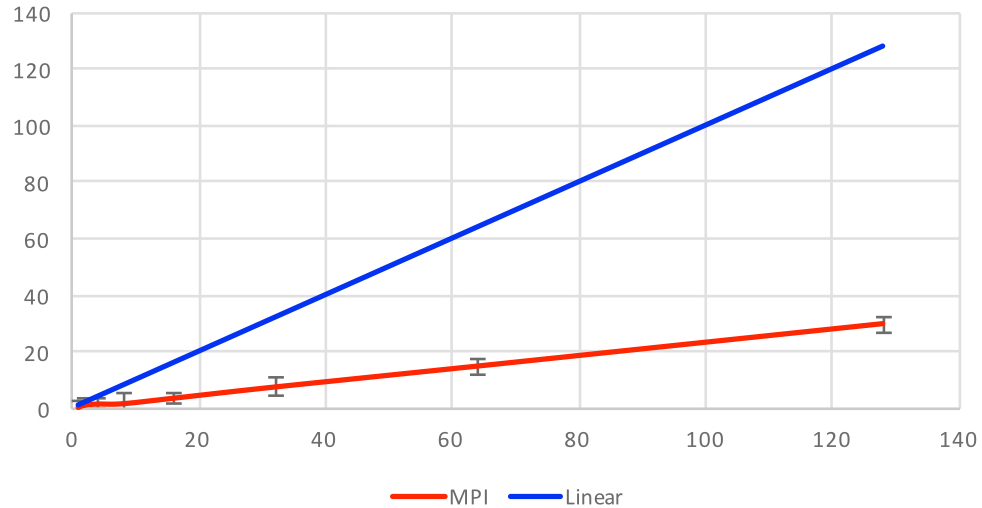
\includegraphics[scale=0.22]{SpeedUp_MPI.jpg}
        \caption{SpeedUp for MPI version}
        \label{SpeedUp_MPI}
    \centering
\end{figure}

\begin{figure}[h!]
    \centering
        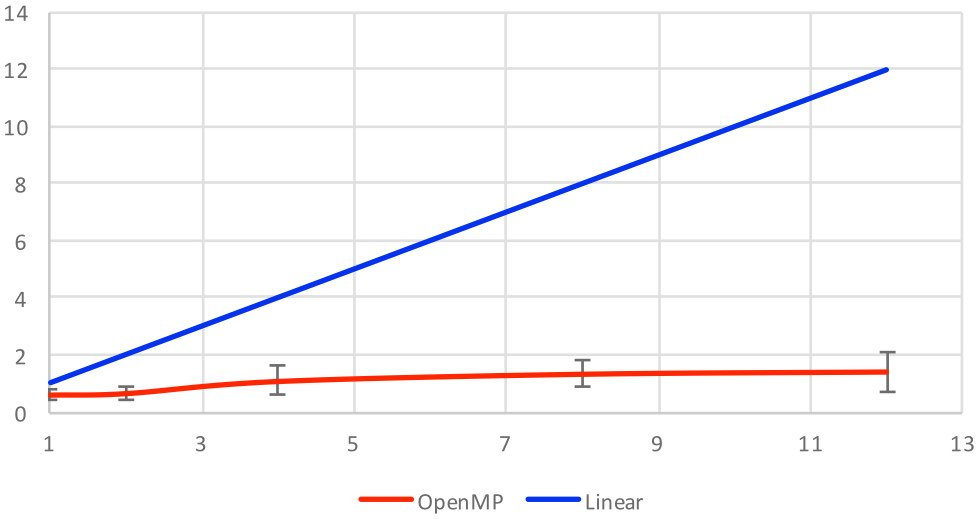
\includegraphics[scale=0.21]{SpeedUp_OpenMP.jpg}
        \caption{SpeedUp for OpenMP version}
        \label{SpeedUp_OpenMP}
    \centering
\end{figure}

We observe that the MPI implementation scales much better as compared to the OpenMP version. For both implementations, we notice that as the processing nodes increases, the difference between theoretical and observed also increases. 

\subsection{Strong Scaling}

In this analysis, we measure how the solution time varies with the number of processors for a fixed problem size. Strong scaling is measured as $\frac{T_{1}}{T_{n}}$ for a given input size, where $T_{1}$ represents the time of the parallel program with 1 node and $T_{n}$ represents the parallel implementation for n inputs.

\begin{figure}[h!]
    \centering
        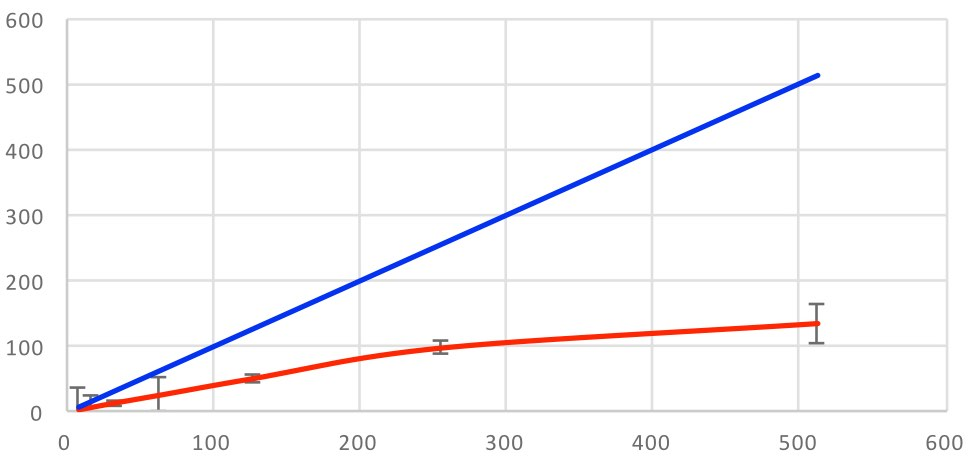
\includegraphics[scale=0.22]{Strong_MPI.jpg}
        \caption{Strong Scaling for MPI version. Measured against 16$\times10^{9}$ inputs.}
        \label{Strong_MPI}
    \centering
\end{figure}

\begin{figure}[h!]
    \centering
        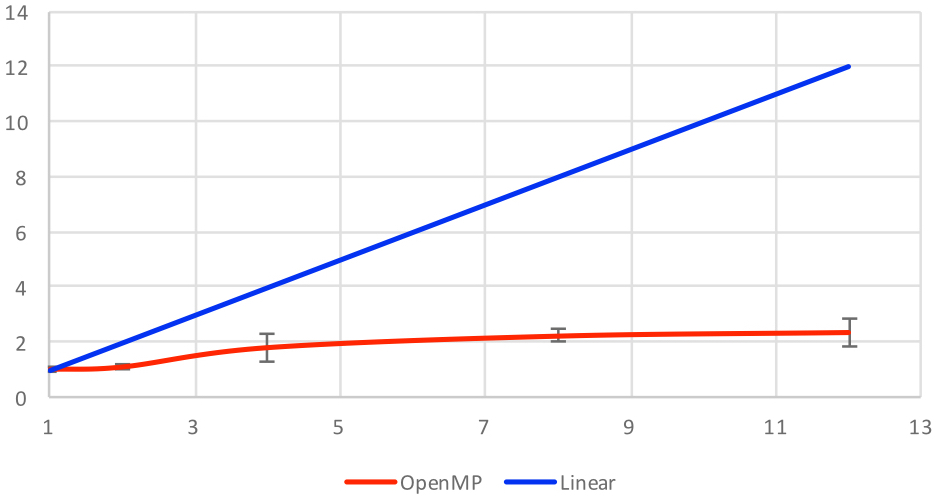
\includegraphics[scale=0.23]{Strong_OpenMP.jpg}
        \caption{Strong Scaling for OpenMP version. Measured against 16$\times10^{9}$ inputs.}
        \label{Strong_OpenMP}
    \centering
\end{figure}

Figure \ref{Strong_MPI} and Figure \ref{Strong_OpenMP} represent the strong scaling characteristics of the MPI and OpenMP versions respectively. The MPI version has better efficiency since it is closer to the constant scale. For both graphs, we observe that the scaling between constant and the respective model deteriorates as the number of processors increases since the communication effects become more pronounced. 

\subsection{Weak Scaling}

In this analysis, we measure how the solution time varies with the number of processors for a fixed problem size per processor. Weak scaling is calculated as the percentage of $\frac{T_{1}}{T_{n}}$ for a given input size per processor, where $T_{1}$ represents the time for 1 node with a fixed input size and $T_{p}$ represents the parallel implementation for the same fixed input size across n nodes.

\begin{figure}[h!]
    \centering
        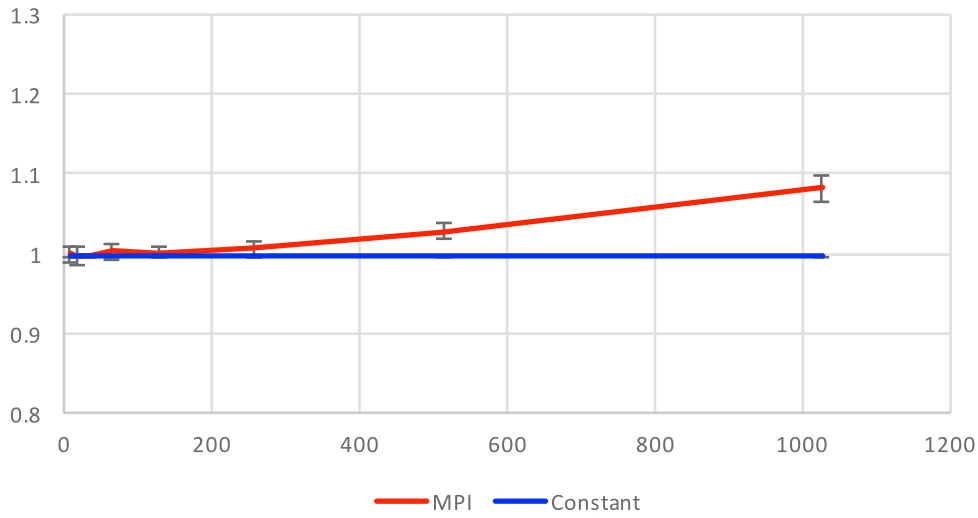
\includegraphics[scale=0.218]{Weak_MPI.jpg}
        \caption{Weak Scaling for MPI version}
        \label{Weak_MPI}
    \centering
\end{figure}

\begin{figure}[h!]
    \centering
        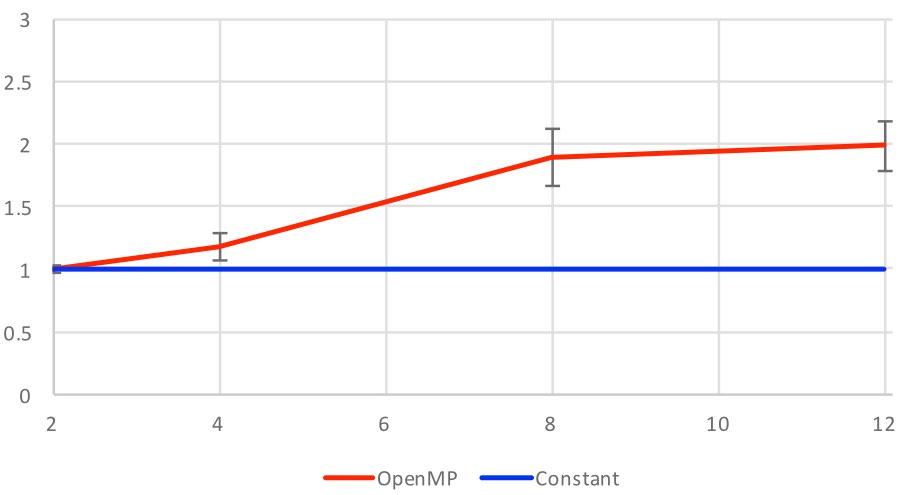
\includegraphics[scale=0.24]{Weak_OpenMP.jpg}
        \caption{Weak Scaling for OpenMP version}
        \label{Weak_OpenMP}
    \centering
\end{figure}

Figure \ref{Weak_MPI} and Figure \ref{Weak_OpenMP} represent the weak scaling characteristics of the MPI and OpenMP versions respectively. We observe that the MPI version scales better since it is closer to the constant scale. For both graphs, we observe that the scaling deteriarates as the number of processors increases since the communication effects become more pronounced. 

\subsection{Big O Constants}

In this analysis, we determine the big-O constants for the three implementations presented above. We plot the ratio between the observed running time of the program versus its theoretical time against a range of input values. From such a graph, we calculate $n_{0}$ and $c$, where $n_{0}$ represents the X-axis region where the plot appears horizontal and $c$ is the Y-axis value at this point. 

\begin{figure}[h!]
    \centering
        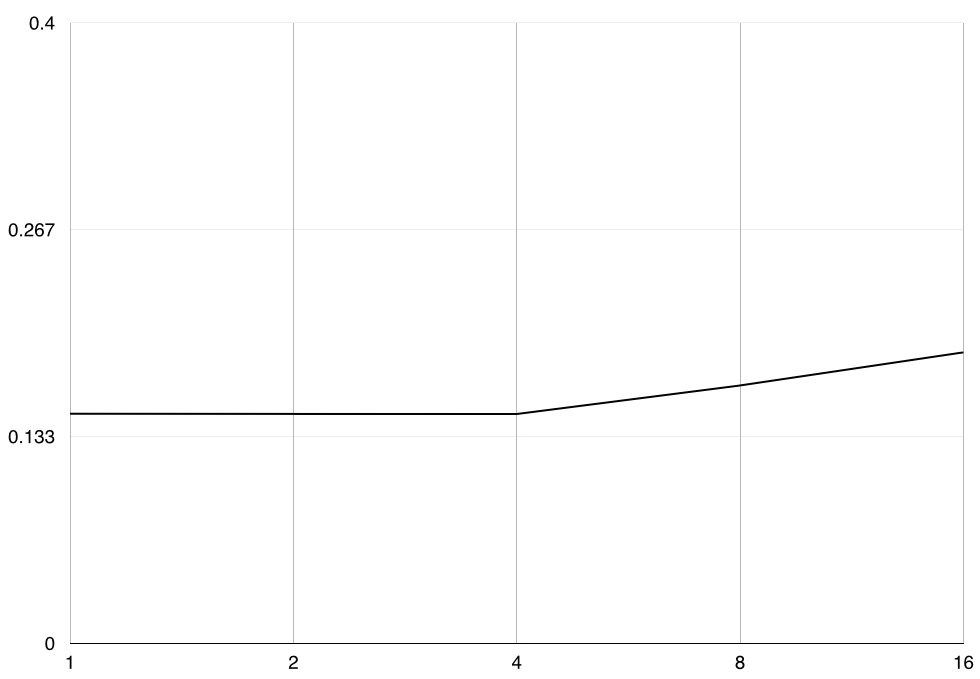
\includegraphics[scale=0.20]{s_1.jpg}
        \caption{Algorithm constants determination for sequential Prefix Sum. The X axis for all figures represents $10^{9}$ integers and the Y axis represents seconds.}
        \label{Seq_c}
    \centering
\end{figure}

Figure \ref{Seq_c} represents such a graph for the sequential implementation of Prefix Sum. We notice that $n_{0} \approx 10^{4}$ and $c \approx 0.147$.

Figure \ref{fig:C4} to Figure \ref{fig:C12} represents such a graph for the OpenMP implementation. Similar to the sequential program graph, we observe that $n_{0} \approx 4\times10^{9}$. However, unlike the sequential program graph, we observe that the $c$ varies. This is explained by the communication overhead imposed as we increase the number of threads, as well as the thread-fork and join time. 

As seen in Section 2.4, the complexity of the parallel prefix sum algorithm is 
\[O\bigg(\frac{n}{p}\bigg) + O(\log p)\]However in practice, we see that an additional cost $F(p)$ (where p is the number of processing nodes) is imposed on the program runtime. As the number of processing nodes increases, so does the cost associated with this function. The analysis of this extra overhead is complicated and varies significantly from system to system. $F(p)$ was observed to vary as 0.2$\times$p. For the particular implementation in OpenMP, we see that $c \approx 0.4$.

Figure \ref{fig:M4} to Figure \ref{fig:M16} represents such a graph for the MPI implementation. We observe that $n_{0} \approx 4\times10^{9}$ and similar to our reasoning for OpenMP, $c \approx 0.2$. $F(p)$ was observed to vary as 0.05$\times$p. We notice that $F(p)$ has a smaller constant factor than the OpenMP implementation since process startup time was ignored.

\section{Future Work}
We observe that the MPI implementation of Prefix Sum is not the most work-optimal solution amongst the two implementations. The algorithm was chosen mainly because of the difficulty in implementing the Balanced scan approach for processing nodes $\neq$ powers of two. The OpenMP implementation avoids this problem through clever use of shared memory. In future work, the MPI implementation can be improved as well.


\section{Conclusion}
Three Prefix sum algorithms were implemented - Sequential, Parallel OpenMP and Parallel MPI. Each of these three implementation used a different algorithm and the performance across them were compared. The source code for all implementation as well as experimental results are available at \href{https://github.com/arunxls/PrefixSum}{github.com/arunxls/PrefixSum}.

\subsection{Sequential}

In terms of program complexity, the sequential algorithm was the simplest. However, the running time is proportional to input size and quickly degrades in performance in comparison to both the parallel implementations.

\subsubsection{MPI}

It was observed that the MPI version scaled best and had the most optimal solution. However, the MPI solution did not include process start up time in this analysis. This could prove to be a significant overhead and might influence a user's preference in choosing a particular implementation. MPI also works well across a distributed compute cluster, something which neither of the other two implementation can do. However, one major disadvantage of using MPI is the need to re-write a significant portion of the program since we don't have the luxury of shared memory. This could prove to a big deciding factor when choosing a particular implementation. 

\subsubsection{OpenMP}

The OpenMP version also gave significant improvements in performance as compared to the sequential version. However, in comparison to the MPI version, we note that the performance does not scale as well. This can be explained by the fact that the OpenMP implementation included in its timing analysis the time taken to start and stop threads, which turns out to be a significant overhead. When this overhead was ignored, it was noticed that the performance scaled much better. Another disadvantage of OpenMP is that it is limited to a single processing node since it relies on shared memory. For large inputs and complex programs, OpenMP might not be the best implementation to choose. One advantage, however, of OpenMP over MPI is in its simplicity. A given sequential program can be much more easily converted to a parallel version using OpenMP. 

\end{document}